% !TeX root = ../main.tex
\chapter{模型构成}\label{ch4}

深度模型只不过是复杂的张量计算,最终可以用线性代数和数学分析分解为标准数学运算。多年来,该领域开发了大量语义清晰的高级模块以及由这些模块组合而来的复杂模型,这些模型已被证明在特定应用领域非常有效。

经验证据和理论结果表明,更深的架构(即长映射组合)可以获得更好的表现。正如我们在 \ref{sec3.4} 节中看到的,由于\keyterm{梯度消失},训练这样的模型具有挑战性,而多项重要技术贡献缓解了这个问题。

\section{层的概念}\label{sec4.1}

我们将那些被设计出来并通过经验认定为通用且高效的标准复杂复合张量操作称为\keyterm{层}。这些层通常包含可训练参数,并且对于设计和描述大型深度模型来说,它们提供了一个便捷的粒度级别。这个术语来源于简单多层神经网络,尽管现代模型可能采用此类模块的复杂图形形式,并包括多个并行路径。

\begin{figure}[h]
    \centering
    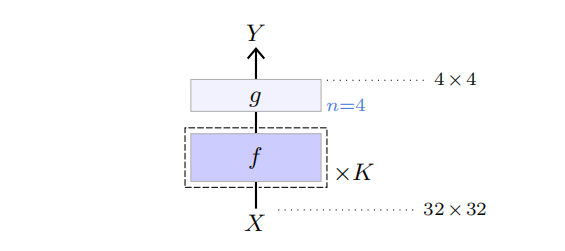
\includegraphics[width=0.9\textwidth]{fig/fig4.0.png}
\end{figure}

在接下来的几页中,我将遵循上面所示模型绘制的约定:

\begin{itemize}
    \item 运算符/层被绘制为框,
    \item 深色表示嵌入了可训练的参数,
    \item 没有默认值的元参数用蓝色字添加在右侧,
    \item 带有乘法因子的虚线外框表示一组层按顺序复制,每个层都有自己的一组可训练参数(如果有的话),
    \item 在某些情况下,当输出维度与输入维度不同时,会在右侧标明。
\end{itemize}

此外,具有复杂内部结构的层会用高度更高的框来表示。

\section{线性层}\label{sec4.2}

就计算和参数数量而言,最重要的模块是\keyterm{线性层}。它们得益于数十年来在矩阵运算算法和芯片设计方面的研究与工程进步。

请注意,在深度学习中,``线性''这一术语通常不恰当地指代\keyterm{仿射运算},即一个线性表达式和一个常数偏置之和。

\subsubsection*{全连接层}

最基本的线性层是\keyterm{全连接层},由大小为 $D' \times D$ 的可训练权重矩阵 $W$ 和维度为 $D'$ 的偏置向量 $b$ 参数化。它实现了泛化到任意张量形状的仿射变换,其中补充的维度被解释为向量索引。形式上,给定维度为 $D_1 \times \dots \times D_K \times D$ 的输入 $X$,它计算出维度为 $D_1 \times \dots \times D_K \times D'$ 的输出 $Y$,其中
\begin{align*}
    \forall d_1,\dots,d_K&,\\
    Y[d_1&,\dots,d_K] = WX[d_1,\dots,d_K]+b
\end{align*}
虽然乍看之下,这种仿射运算似乎仅限于旋转、对称和平移等几何变换,但实际上它能做的远不止这些。特别是,用于降维或信号过滤的投影,而且,从点积作为相似性度量的角度来看,矩阵-向量乘积可以解释为计算输入向量所编码的查询与矩阵行所编码的键之间的匹配得分。

正如我们在 \ref{sec3.3} 节中看到的,梯度下降从\keyterm{参数的随机初始化}开始。如果这一操作做得过于简单,如 \ref{sec3.4} 节所示,网络可能会遭受激活和梯度爆炸或消失的影响 \citep{glorot10a}。深度学习框架实现了初始化方法,特别是按照输入的维度来缩放随机参数,以保持激活的方差恒定并防止病态行为。

\subsubsection*{卷积层}

线性层可以将任意形状的张量通过重塑成向量的方式作为输入,只要它具有正确数量的系数即可。然而,这样的层不太适合处理大型张量,因为参数数量和操作数量与输入和输出维度的乘积成正比。例如,要处理一个大小为 $256 \times 256$ 的 RGB 图像作为输入并计算相同大小的结果,将需要大约 $4 \times 10^{10}$ 个参数和乘法运算。

除了这些实际问题之外,大多数高维信号都是强结构化的。例如,图像在平移、缩放和某些对称性方面表现出短期相关性和统计平稳性。这并没有反映在全连接层的\keyterm{归纳偏置}中,它完全忽略了信号结构。

为了利用这些规律,首选的工具是\keyterm{卷积层}。卷积层同样是仿射的,但它局部处理时间序列或二维信号,并在各处使用相同的操作符。

\keyterm{一维卷积}主要由三个\keyterm{元参数}定义:内核大小 $K$、输入通道数 $D$、输出通道数 $D'$,以及仿射映射 $\phi(\cdot;w):\mathbb{R}^{D \times K} \to \mathbb{R}^{D' \times 1}$ 的可训练参数 $w$。

它可以处理任何大小为 $D \times T$ 且 $T \ge K$ 的张量 $X$,并将 $\phi(\cdot;w)$ 应用于 $X$ 的每个大小为 $D \times K$ 的子张量,将结果存储在大小为 $D' \times (T-K+1)$ 的张量 $Y$ 中,如图 \ref{fig4.1}(左半部分)所示。

\newpage

\begin{figure}[h]
    \centering
    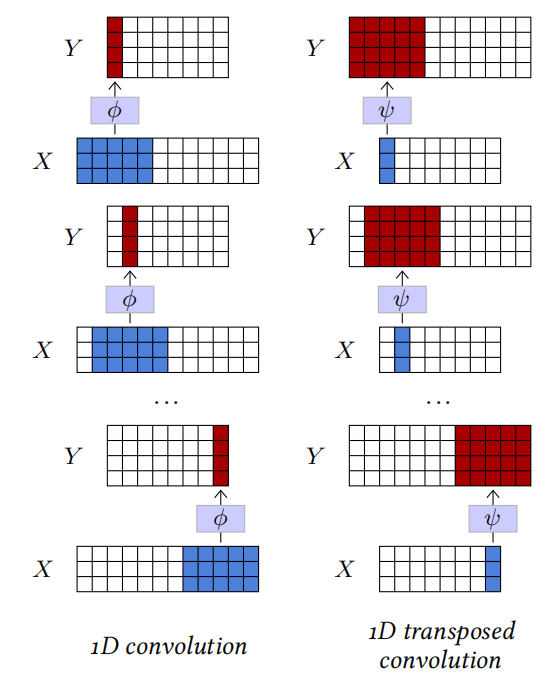
\includegraphics[width=0.9\textwidth]{fig/fig4.1.png}
    \caption[一维卷积]{一维卷积(左)接受 $D \times T$ 张量 $X$ 作为输入,将相同的仿射映射 $\phi(\cdot;w)$ 应用于形状为 $D \times K$ 的每个子张量,并将生成的 $D' \times 1$ 张量存储到 $Y$ 中。一维转置卷积(右)接受 $D \times T$ 张量作为输入,将相同的仿射映射 $\phi(\cdot;w)$ 应用于每个形状为 $D \times 1$ 的子张量,并对移位后的 $D' \times K$ 结果张量求和。两者都可以处理不同大小的输入。}
    \label{fig4.1}
\end{figure}

\keyterm{二维卷积}与之类似,但具有 $K \times L$ 大小的内核,并接受 $D \times H \times W$ 大小的张量作为输入(参见图 \ref{fig4.2},左半部分)。

\begin{figure}[h]
    \centering
    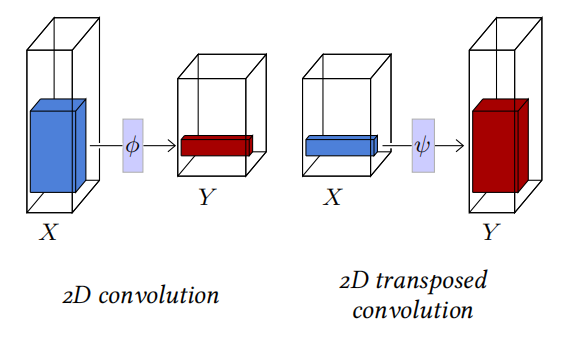
\includegraphics[width=0.9\textwidth]{fig/fig4.2.png}
    \caption[二维卷积]{二维卷积(左)接受 $D \times H \times W$ 张量 $X$ 作为输入,将相同的仿射映射 $\phi(\cdot;w)$ 应用于形状为 $D \times K \times L$ 的每个子张量,并将生成的 $D' \times 1 \times 1$ 张量存储到 $Y$ 中。二维 转置卷积(右)接受 $D \times H \times W$ 张量作为输入,将相同的仿射映射 $\phi(\cdot;w)$ 应用于每个形状为 $D \times 1 \times 1$ 的子张量,并对移位后的 $D' \times K \times L$ 结果张量求和得到 $Y$。}
    \label{fig4.2}
\end{figure}



这两种操作的可训练参数都是 $\phi$ 的参数,可以分别将其设想为大小为 $D \times K$ 或 $D \times K \times L$ 的 $D'$ 个\keyterm{过滤器},以及一个维度为 $D'$ 的\keyterm{偏置向量}。

这样的层对平移是\keyterm{等变}的,这意味着如果输入信号被平移,输出也会以类似的方式变换。当处理其分布对于平移不变的信号时,此属性会产生理想的\keyterm{归纳偏差}。

卷积层还接受三个额外的\keyterm{元参数},如图 \ref{fig4.3} 所示:

\begin{itemize}
    \item \keyterm{填充}指定在处理输入张量之前应在输入张量周围添加多少个零系数,特别是在内核大小大于 $1$ 时维持张量尺寸。其默认值为 $0$。
    \item \keyterm{步幅}指定在处理输入时使用的步长,允许通过使用大步长以几何方式减小输出大小。其默认值为 $1$。
    \item \keyterm{膨胀}指定局部仿射操作符的过滤器系数之间的索引计数。其默认值为 $1$,更大的值对应于在系数之间插入零,这会增加过滤器/内核的大小,同时保持可训练参数数量不变。
\end{itemize}

\begin{figure}
    \centering
    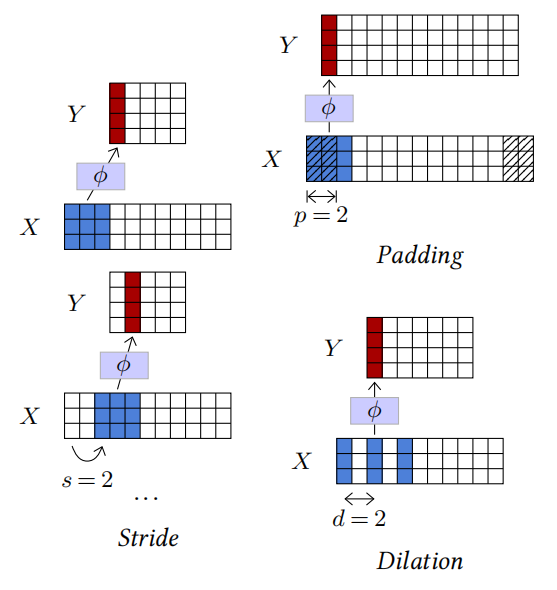
\includegraphics[width=0.9\textwidth]{fig/fig4.3.png}
    \caption[步长、填充和膨胀]{除了内核大小和输入/输出通道数之外,卷积还接受三个元参数:步长 $s$(左)在经过输入张量时调节步长,填充 $p$(右上)指定在处理输入张量之前在输入张量周围添加多少个零元素,膨胀 $d$(右下)参数化过滤器系数之间的索引计数。}
    \label{fig4.3}
\end{figure}

除了通道数之外,卷积的输出通常小于其输入。在没有填充或膨胀的一维情况下,如果输入的大小为 $T$,内核的大小为 $K$,步幅为 $S$,则输出的大小为 $T' = (T - K)/S + 1$。

\newpage

给定由卷积层计算的激活,或某个位置上所有通道的值向量,它所依赖的输入信号部分称为其\keyterm{感受野}(见图 \ref{fig4.4})。与 $D \times H \times W$ 激活张量的单个通道对应的 $H \times W$ 子张量之一称为\keyterm{激活图}。

\begin{figure}
    \centering
    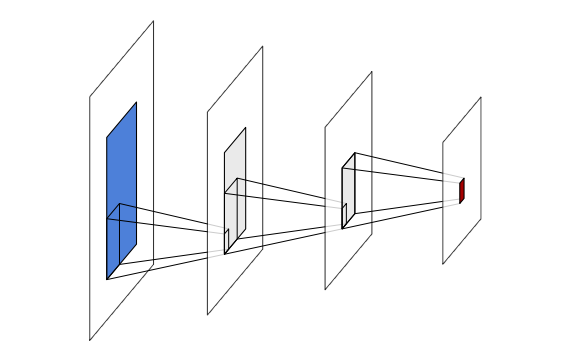
\includegraphics[width=0.9\textwidth]{fig/fig4.4.png}
    \caption[感受野]{给定一系列卷积层(这里为红色)中的激活,其\keyterm{感受野}是输入信号(蓝色)中调节其值的区域。每个中间卷积层大约按照核的宽度和高度增加该区域的宽度和高度。}
    \label{fig4.4}
\end{figure}

卷积用于重新组合信息,通常是为了减少表示的空间大小,以换取更多数量的通道,从而转化为更丰富的局部表示。它们可以实现微分运算符,例如边缘检测器或模板匹配机制。一系列这样的层也可以视为一种组合和分层表示 \citep{arxiv-1311.2901},或者作为一个扩散过程,其中信息在穿过层时可以通过内核大小的一半进行传输。

逆运算是\keyterm{转置卷积},也由局部仿射运算符组成,由与卷积类似的元和可训练参数定义,例如,在一维情况下,它将一个仿射映射 $\phi(\cdot;w):R^{D \times 1} \to R^{D' \times K}$ 应用于输入的每个 $D \times 1$ 子张量,并将移位后的 $D' \times K$ 结果张量求和以计算其输出。这样的操作符增加了信号的尺寸,直观上可以理解为一个合成过程(见图 \ref{fig4.1} 和图 \ref{fig4.2} 的右半部分)。

一系列卷积层是将大维度信号(如图像或声音样本)映射到低维张量的常用架构。例如,这可以用来获取用于分类的类别分数或压缩表示。转置卷积层以相反的方式用来从压缩表示构建大维度信号,要么是为了评估压缩表示是否包含足够的信息来重构信号,要么是为了合成,因为在低维表示上学习密度模型更容易。我们将在 \ref{sec5.2} 节中重新讨论这个话题。

\section{激活函数}\label{sec4.3}

\section{池化}\label{sec4.4}

\section{Dropout}\label{sec4.5}

\section{归一化层}\label{sec4.6}

\section{跳跃连接}\label{sec4.7}

\section{注意力层}\label{sec4.8}

\section{代币嵌入}\label{sec4.9}

\section{位置编码}\label{sec4.10}